\section{Overview of Sensibility Testbed}\label{sec-overview}
%Here we are going to put the overview and high-level walkthrough. 
%(I'm putting the old Section 3.3 here for now. )
The design of \sysname is guided by three design principles. In this 
section, we describe these principles and the resulting testbed 
components. We also show the testbed operation via two usage 
scenarios.

\subsection{Design Principles}\label{sec-overview}

\begin{figure}
\center{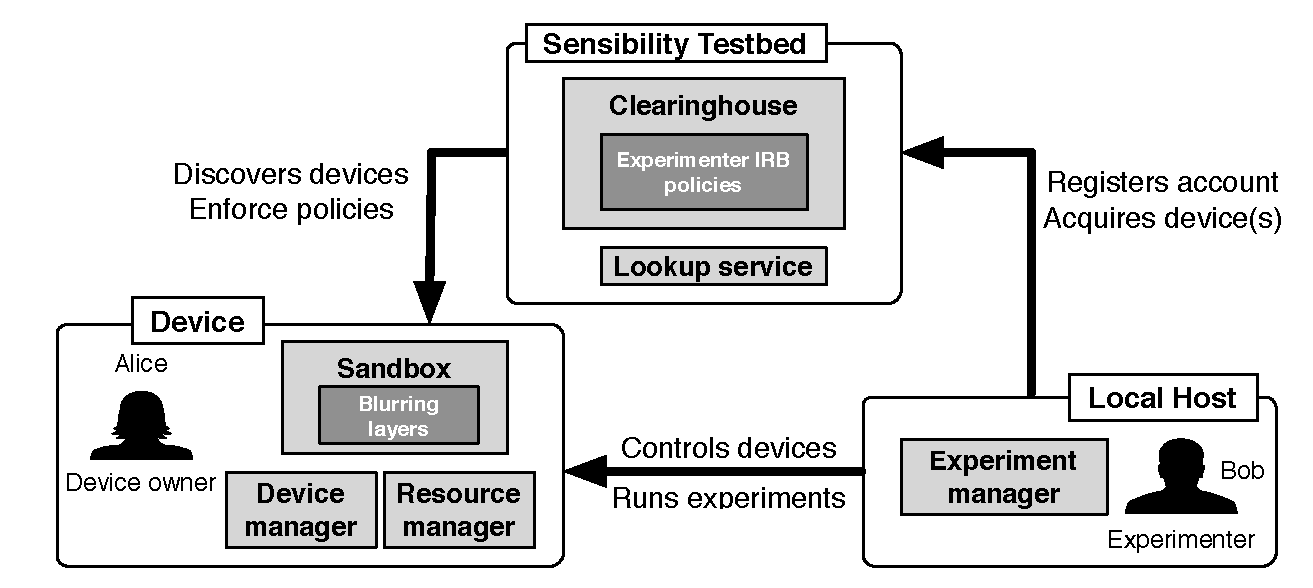
\includegraphics[width=\columnwidth]{figs/arch.pdf}}
%\vspace*{-20pt}
\caption{\small Sensibility Testbed architecture. \label{fig-arch}}
\end{figure}

%\subsubsection{Interacting Parties}\label{sec-parties}
The operation of Sensibility Testbed  involves three types of interacting
parties, as shown in Figure~\ref{fig-arch}: mobile \textit{devices} 
owned by ordinary people, with our app installed; a 
\textit{clearinghouse} server that discovers and configures
participating devices; and \textit{experimenters} who want to run
experiments on mobile devices. The interaction between these three 
components, as illustrated in Figure~\ref{fig-arch}, is designed to 
support three fundamental design principles.
%\subsubsection{Testbed Architecture}

\textbf{Shared access to device resources.} 
Since hardware resources are limited on mobile devices, it is 
not possible to dedicate an entire device to an experiment. Therefore, 
Sensibility Testbed allows several experiments to share one device. It 
uses a sandbox to isolate one researcher's code from 
 another, through its performance isolation technique. The sandbox 
also prevents experiment code from inadvertently harming the device
via security isolation. Other software within the device controls a
researcher's access to a sandbox, allows the device 
owner to opt in or out of the testbed, and allows the device
to communicate with the rest of the testbed. Together, they form the
\textit{device software} (Section~\ref{sec-repy}, though only the 
sandbox is shown in Figure~\ref{fig-arch}).

\textbf{A centralized way of allocating devices and mediating data access.}
Sensibility Testbed is designed to provide both enhanced security and 
more efficient management of experimental setup, so another principle 
for the design was a central component that could serve as a a trusted 
intermediary for acquiring and managing device resources. Both tasks 
are delegated to  a server called \textit{clearinghouse}~\cite{ch}. The 
clearinghouse allows researchers to 
register accounts for each experiment, and share access to a common 
pool of devices, freeing them from the need to individually recruit participants. 
The clearinghouse can also allocate resources and mediate 
data access according to policies defined by a researcher's IRB. The 
clearinghouse thus facilitates device sharing and policy enforcement 
(Section~\ref{sec-ch}).

\textbf{Local support for remote experimentation.} 
The last design principle was to allow researchers to manage their 
experiments on remote devices from a local machine, as is offered 
by other testbeds~\cite{hibler2008large, peterson2006experiences}. Sensibility 
Testbed addresses this need by using a tool called \textit{experiment 
manager}. The experiment manager provides access to 
hardware resources on mobile devices using the researcher's testbed 
credentials (assigned by the clearinghouse). This tool will be introduced
in Section~\ref{sec-emt}.

\smallskip
The following section describes %the three components in more detail, and 
%addresses 
how these parties interact to enable safe experimentation on mobile devices. 


\subsection{Testbed Operation}


The basic operation of Sensibility Testbed involves two separate 
parties: a device owner interested in participating in experiments 
and a researcher seeking to run tests on remote devices. The 
device owner starts by installing the Sensibility Testbed app from 
the Android app store~\cite{sensibility-app}, which includes all the 
device software (Section~\ref{sec-repy}). After downloading the app, 
the device owner is informed about the testbed's general usage policy 
in a consent form and must give consent before participating.
Any device owner, regardless of age, country, or background, can 
opt into our testbed in this manner, and can opt out just by uninstalling 
the app. The app will also display a list of experiments and each 
experiment's policies, so the owner can opt out of individual experiments. 

To conduct an experiment, a researcher will first provide his institution's 
IRB policies to the clearinghouse and will sign up for his experiment. \yanyan{need a screenshot} 
The clearinghouse server helps him acquire devices, and codifies 
policies specified by the researcher's IRB. After obtaining remote devices, 
the researcher can perform experiments directly on the devices through 
the experiment manager, using the credentials assigned by the clearinghouse. 



%Device owners like Alice participate in Sensibility Testbed by p.

%These policies restrict what and how data can be accessed by the 
%researcher. 
%into data blurring layers that are enforced on
%mobile devices. Such a process can protect device
%owners' personal information. 
%Researchers' code runs in a sandbox that isolates the code from the 
%rest of the device host system. 
%To control the execution of code, Bob uses his own 
%desktop or laptop computer to manage the 
%experiments via the experiment manager. It deploys 
%and runs experiments in sandboxes on remote devices that are 
%acquired through the clearinghouse.

%\textbf{Usage scenario 1: Smartphone owner volunteers as a testbed participant.}
%Alice downloads the Sensibility Testbed app from the Google Play 
%Store~\cite{sensibility-app}, which will install Repy and other software on her phone.
%The app displays a consent form, \yanyan{cite link} containing the testbed's 
%general usage policy. Alice must review and must agree to this 
%policy before installation. If Alice gives her consent, her device will be 
%installed with the Repy sandbox, the native Android code to 
%start or stop the sandbox, and an interface to communicate with the testbed 
%infrastructure (particularly the clearinghouse, described below). 
%By agreeing to our general usage policy, any device 
%owner, regardless of age, country, or background, need only to opt into our testbed as a
%volunteer \textit{once}, at the time of app installation. 
%%As a result, an 
%%researcher like Bob who wants to conduct an experiment 
%%%requests devices through our clearinghouse, which assigns 
%%%them devices from a set of available resources. As a result, 
%%%the researcher
%%does not need to get consent from each subject for each individual
%%experiment. \lois{is the previous sentence needed? I don't think so} 
%The testbed thus greatly simplifies the process for both the 
%device owners and experimenters. 

Two usage scenarios further illustrate how the clearinghouse 
protocol in operation, are given below. In this case, 
Alice, a device owner, participates in the testbed. A researcher, Bob, 
runs code on Sensibility Testbed using Alice's smartphone, discovered among other
devices. Specifically, Bob wants to know the cellular service
quality in major cities. As such, he needs location information
of individual devices, their cellular service provider, network
type (3G, 4G, LTE, etc.), and signal strength. 

\subsubsection{Clearinghouse tracks devices}\label{sec-case1}
Once the app is started, Alice's device can be discovered by 
the clearinghouse. The resource manager in her app periodically contacts 
a lookup service to advertise the device sandbox to the rest of the testbed, 
such as the clearinghouse or experiment manager. \yanyan{resource 
manager and lookup service have not been introduced yet.}
A lookup service is a distributed key-value store, such as a 
distributed hash table (DHT)~\cite{dht}, that allows one to associate 
keys with values and retrieve values associated with keys. In this case, 
Alice's resource manager uses an \textit{identification key}, \path{key.alice}, 
generated during the app installation, and associates this key 
with Alice's device IP address and port number, by 
storing this key-value entry in the lookup service. This key is not 
associated with Alice or her device's identity, but only with the app's 
installation on the device. 
%When the clearinghouse knows Alice's key, it can retrieve Alice's 
%IP:port by looking up her key, \path{key.alice}, through 
%the lookup service. With IP:port, the clearinghouse can then
%communicate with Alice's device over the network.
\yanyan{I think the device first puts key.sensibility 
in the lookup service. is this key's value key.alice? so when the 
clearinghouse looks up key.sensibility, it finds out key.alice; and then
it uses key.alice to lookup IP:port. But is it necessary to go into such detail?}

%The app interface also displays a list of experiment running
%on Alice's device, and their policies. Therefore, 
%through the app interface, Alice may uninstall, or 
%choose to opt out of individual experiments. 
%\lois{how? I have not seen this explained yet and I think its critical to discuss this}

To keep track of Alice's device, the
clearinghouse periodically queries the lookup service to
discover any new device installs. Once Alice's device is discovered, the
clearinghouse obtains \path{key.alice}, and thus
%clearinghouse uses a database that stores her device's unique
%identification key, \path{key.alice}, generated during installation. 
can retrieve Alice's  IP address and port number by 
looking up her key in the lookup service. This allows the clearinghouse
to communicate with Alice's device over the network.
If Alice uninstalls the Sensibility Testbed app, 
\path{key.alice} is deleted at the clearinghouse, which effectively unlinks
her device from any metadata stored on the clearinghouse. The key
will also be removed from the lookup service after a period of inactivity.
An experiment manager controlled by a researcher can lookup
available device installs in a similar way. Instead of finding all devices
available to the testbed, the experiment manager will only be able to 
lookup devices assigned to the researcher by the clearinghouse.

%The clearinghouse
%plays an intermediate role between the experimenter and 
%the device owner.
%As described in Section~\ref{sec-overview}, when an 
%experimenter registers at the clearinghouse, he
%needs to provide his IRB policies. These policies ensure that
%the researcher cannot conduct experiments to access data that
%extend beyond the experiment policy. The clearinghouse 
%translates and codifies each policy, and instructs the 
%sandboxes on remote devices to implement these policies. 
%When experiment code is running in the sandbox, the 
%policies will be applied to restrict %the precision of sensor 
%%data or the frequency to access 
%sensor access. 

\subsubsection{Researcher registers experiment and provides IRB policies}
\label{sec-case2}
 Researcher Bob's first step to access the testbed begins when he
%needs to provide a set of etailed IRB policies from his institution. 
%In order to obtain an IRB approval, a researcher first 
%To do this, Bob 
fills out an experiment registration form at the 
clearinghouse. The clearinghouse registration page shows 
a list of sensors accessible to testbed users, and 
each of their possible accuracy and access frequency limits. 
%\lois{I think I already asked this, but is it literally just the sensors that the page shows, and not the devices containing the sensors that are shown? It's a small point, but I think it has to be clarified} 
In this particular case, Bob specifies that 
%what data can be accessed by a research experiment, at which 
%granularity or frequency such data can be accessed, how data 
%should be securely stored, and so on. \yanyan{cite register 
%experiment website url.}
his experiment can (1) read location information
from devices at the granularity of a city, (2) read accurate
cellular signal strength and network type, as well as
%but not allow access to information about 
cell IDs, and (3) get location and
cellular network data updates every 10 minutes. 
%Bob submits an
%experiment description for these requirements, which the
%clearinghouse will codify into policies that are later enforced
%on remote mobile devices (Section~\ref{sec-ch}).
%Bob then uses this form, along with other forms downloaded 
%from the clearinghouse, to apply for IRB approval at his institution.
%
After filling out this form, Bob downloads the experiment description 
he provided, the detailed information about Sensibility Testbed and 
several relevant forms, such as 
those addressing consent, terms of participation (for device owners),  
terms of usage (for the researcher), and so on. \yanyan{cite our docs}  
Bob then uses these forms as a template to complete the IRB application 
with his institution. These forms serve as a set of reference documents 
to make it easier for researchers like Bob to 
file the necessary IRB paperwork with their institutions.

After the application is submitted, Bob's IRB may disagree with 
his initial experiment requirements. For example, Bob's IRB will not permit
his experiment to access cell IDs in cellular networks, but 
approves the other policies. 
%Bob wants to access cell 
%IDs in cellular networks, but his IRB disallows such data access. Bob then
In this case, Bob will revise the experiment registration form, refile the paperwork, 
and obtain IRB approval. Bob then submits the revised  
registration form and his IRB approval to the clearinghouse.

Finally, the clearinghouse
parses Bob's registration form, extracts each data accuracy and access 
frequency limits approved by Bob's IRB policies (to blur an exact location 
to a city center, disallow access to cell IDs, and allow cellular network and 
location query once every 10 minutes), and assigns an experiment 
account to Bob. Once his account is activated, 
%Bob obtains his \textit{authentication keys} assigned by the 
%clearinghouse. These keys are to authenticate Bob with the 
%clearinghouse and the set of devices to which he has access.
%\path{bob.public} and \path{bob.private}. Next, 
Bob obtains his public/private key pair, and can request a number of devices from the 
clearinghouse (Section~\ref{sec-ch}). The clearinghouse then looks up
available devices like in Section~\ref{sec-case1}. If the clearinghouse 
discovers that Alice's device is available, it
assigns her device to Bob's experiment account by placing Bob's
public key in Alice's sandbox. At this point, Bob can access Alice's 
device through his experiment manager, just like using \texttt{ssh}.

As already described, the clearinghouse has a default set of blurring layers 
for accuracy and access frequency levels for each sensor. 
The clearinghouse first instructs 
the sandbox on Alice's device to add Bob's policies by preloading
a set of blurring layer code. It then supplies the extracted data from 
Bob's registration form as input parameters to the blurring layers. 
%that will be instantiated on Alice's device. 
When Bob runs his experiment, the policies are transparently applied
to the experiment code. 
The policies are easily customizable. Details about
how policies are implemented will be introduced in Section~\ref{sec-policy}.

%\textbf{Usage scenario 4: Researcher acquires device(s) and runs an experiment.}
%\label{sec-acquire-run}
%The above clearinghouse protocol ensures the enforcement of data
%access policies. Additionally, 
%To perform an experiment, Bob needs to request the use of some devices. 
%Recall that a testbed-specific key, \path{key.sensibility}, is distributed
%with the Sensibility Testbed app downloaded and installed by device
%owners (Section~\ref{sec-owner-participate}). 
%
%\yanyan{Albert thinks this is too much detail.}
%At this moment,  Bob has obtained an account with the clearinghouse.
%and is assigned a pair of public and 
%private keys, \path{key.bob-pub} and \path{key.bob-priv}, by the
%clearinghouse. 
%If the clearinghouse finds that Alice's device is available from the 
%lookup service, it
%%adds Bob's public key, \path{key.bob-pub}, to
%%the sandbox on Alice's device. This indicates that Bob is
%%authorized to use this sandbox on Alice's device, and 
%assigns Alice's device to Bob's experiment account by placing Bob's
%public key on Alice's device. It then instructs 
%the sandbox on Alice's device to add Bob's policies by preloading
%a set of blurring layer code. At this point, Bob can access Alice's 
%device through the experiment manager, just like using \texttt{ssh}.
%Bob writes his experiment 
%code in the Python-like language supported by our secure sandbox.
%The following is a snipet of code that gets location coordinates 
%from a device:
